\documentclass[conference]{IEEEtran}
\IEEEoverridecommandlockouts
% The preceding line is only needed to identify funding in the first footnote. If that is unneeded, please comment it out.
\usepackage{cite}
\usepackage{amsmath,amssymb,amsfonts}
\usepackage{algorithmic}
\usepackage{graphicx}
\usepackage{textcomp}
\usepackage{xcolor}
\usepackage{hyperref}
\usepackage{float}
\def\BibTeX{{\rm B\kern-.05em{\sc i\kern-.025em b}\kern-.08em
    T\kern-.1667em\lower.7ex\hbox{E}\kern-.125emX}}
\begin{document}

\title{Unblock Me}

\author{\IEEEauthorblockN{Guilherme Silva (201603647)}
\IEEEauthorblockA{\textit{IART} \\
\textit{FEUP}\\
Porto, Portugal \\
up201603647@fe.up.pt}
\and
\IEEEauthorblockN{Miguel Duarte (201606298)}
\IEEEauthorblockA{\textit{IART} \\
\textit{FEUP}\\
Porto, Portugal \\
up201606298@fe.up.pt}
\and
\IEEEauthorblockN{Rui Alves (201606746)}
\IEEEauthorblockA{\textit{IART} \\
\textit{FEUP}\\
Porto, Portugal \\
up201606746@fe.up.pt}
}

\maketitle

\begin{abstract}
The aim of this paper is to implement and compare Artificial Intelligence algorithms for solving the game Unblock Me, in which rectangular pieces block the path of a red special piece. The objective of the game is for the special piece to reach the exit of the level, which is achieved by moving it and the other pieces.
The problem will be described and then formulated as a \textit{Search Problem}, together with some discussion on the reasoning behind some of the decisions taken during this process.
Several algorithms will be investigated, along with testing them against levels with varying difficulty and branching factors. Both the efficiency in reaching a solution and the cost of the calculated solution will be taken into account in the pursuit for the optimal \textit{Search Algorithm}.
{\huge NEEDS PART ABOUT SECTION V THAT WILL BE CHANGED}

\end{abstract}

\begin{IEEEkeywords}
Artificial Intelligence, Search Problems, Path finding algorithms, Graph Algorithms, DFS, BFS, Iterative Deepening, Greedy Search, A*, Bi-directional Search
\end{IEEEkeywords}

\section{Introduction}
The game that is the subject of study in this paper (\textit{Unblock Me}) will be approached with several different \textit{Search Algorithms}, implemented in \textit{Python}, in order to conclude what is the best approach for solving it using \textit{Artificial Intelligence Algorithms}.

Firstly, the game will be described in further detail, ensuring that all non-formal aspects of it are well documented. Secondly, it will be formulated as a \textit{Search Problem}, with the approach taken in doing so being illustrated in increased depth, providing reasoning for the decisions taken. Thirdly, a research on related work on this topic will be presented, giving some insight on the problem from other points of view.
{\huge Finally, a small section covers the conclusions and future work.}

\section{Problem Description}
\textit{Unblock Me} is a puzzle game that was released in 17-06-2009 by \textit{Kiragames}. Each level consists of a 6x6 board, surrounded with walls (except for the puzzle's exit). 

\begin{figure}[H]
    \centerline{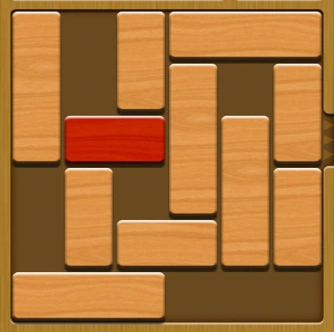
\includegraphics[width=100px]{img1.png}}
    \caption{Example of an \textit{Unblock Me} level}
    \label{fig}
\end{figure}

The game's objective is to move a special piece to the level's exit, by moving that and the other pieces with the least number of movements possible. Pieces are rectangles with a given orientation (vertical or horizontal) and constant length. Pieces can only move in the direction of their orientation into empty cells (they may not overlap).  

\begin{figure}[H]
    \centerline{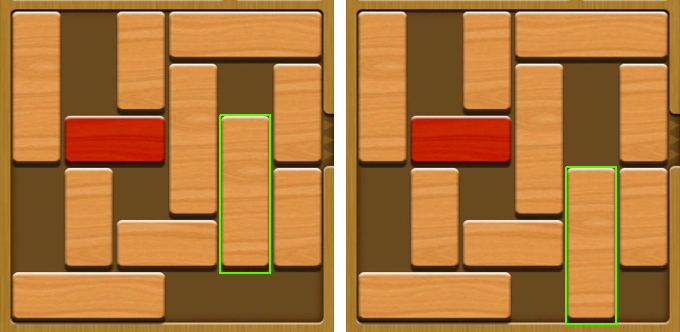
\includegraphics[width=200px]{img2.png}}
    \caption{Piece moving down one cell}
    \label{fig}
\end{figure}

Levels are fully surrounded by walls, except for the level's exit door that is alligned with the special piece and by which only the special piece can go through. The level is completed once the piece goes through the exit door.
 
\begin{figure}[H]
    \centerline{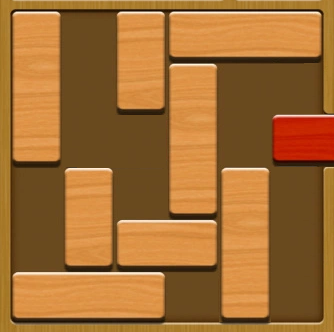
\includegraphics[width=100px]{img3.png}}
    \caption{Beating a level by going through the exit}
    \label{fig}
\end{figure}

Some levels may even contain fixed blocks that can not be moved, representing obstacles.
 
\begin{figure}[H]
    \centerline{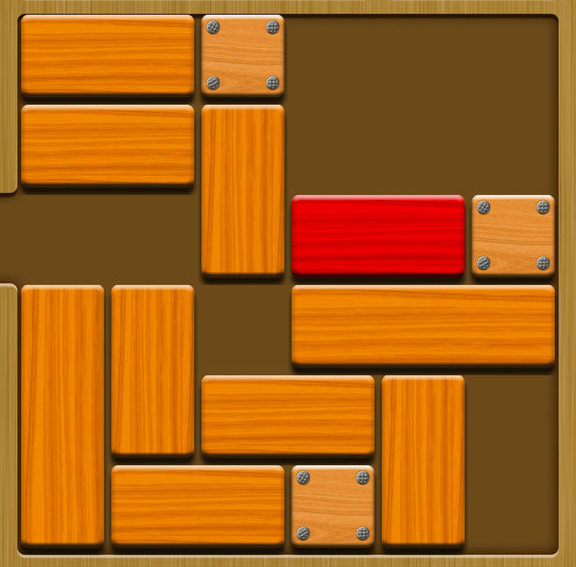
\includegraphics[width=100px]{img4.png}}
    \caption{Example of an \textit{Unblock Me} level containg fixed blocks}
    \label{fig}
\end{figure}

\section{Problem Formulation}
The game's solving process can be formulated as a searching problem, in which the goal is to find the sequence of moves (state transitions) that take the special piece to the level's exit door - the problem's goal state. 

\subsection{Game State Representation} \label{subsec:gr}

\begin{itemize}
        \item List of pieces, where each piece contains the following information:
    \begin{itemize}
        \item Origin Square (top left piece corner, e.g. (0,0))
        \item Length (e.g. 4)
        \item Direction (H or V)
    \end{itemize}
    \item Reference to the special piece
    \item Matrix of booleans, where True means the cell is empty
\end{itemize}

This representation of the game state makes the generation of the valid movements easier, due to the fact that to determine possible movements 
Esta representação do estado do jogo facilita a geração de todos os movimentos válidos, devido ao facto de que o que condiciona o movimento de uma peça não ser necessariamente dependente das outras peças, mas dos espaços vazios do estado atual. Para gerar estes movimentos, basta percorrer a lista de peças, verificando se cada peça possui algum espaço vazio em cada uma das suas duas extremidades (com base na sua orientação). A representação apresentada facilita a execução desta tarefa, tornando-a também pouco custosa (facto importante devido ao elevado número de cálculos deste tipo):
Utilizando uma lista para armazenar todas as peças, é trivial percorrê-la a fim de determinar quais delas se podem mover num dado estado;
Utilizando uma matriz (de valores booleanos, que indicam se uma célula está ou não ocupada) é trivial verificar se as duas células adjacentes às extremidades de uma peça estão ou não vazias
Por fim, a utilização de uma referência para a peça especial permite um acesso constante a essa peça, que será útil para as operações relacionadas com as heurísticas de avaliação.

\subsection{Initial State}
The initial state depends of the level in question, being represented by a game state described in \autoref{subsec:gr}.

\subsection{Goal State}
The goal state consists of a piece configuration where the special piece reaches the level exit.

\subsection{Operators}
\begin{itemize}
    \item Move piece to the left:
    \begin{itemize}
        \item Pre-conditions:
        \begin{itemize}
            \item Piece with horizontal orientation
            \item Cell that is adjacent to the piece's left extremity must be empty
        \end{itemize}
        \item Results: The pieces position moves one cell to the left
        \item Cost: 1 movement
    \end{itemize}
    \item Move piece to the right:
    \begin{itemize}
        \item Pre-conditions:
        \begin{itemize}
            \item Piece with horizontal orientation
            \item Cell that is adjacent to the piece's right extremity must be empty
        \end{itemize}
        \item Results: The pieces position moves one cell to the right
        \item Cost: 1 movement
    \end{itemize}
    \item Move piece up:
        \begin{itemize}
        \item Pre-conditions:
        \begin{itemize}
            \item Piece with vertical orientation
            \item Cell that is adjacent to the piece's top extremity must be empty
        \end{itemize}
        \item Results: The pieces position moves one cell up
        \item Cost: 1 movement
    \end{itemize}
    \item Move piece down:
    \begin{itemize}
        \item Pre-conditions:
        \begin{itemize}
            \item Piece with vertical orientation
            \item Cell that is adjacent to the piece's bottom extremity must be empty
        \end{itemize}
        \item Results: The pieces position moves one cell down
        \item Cost: 1 movement
    \end{itemize}
\end{itemize}

\subsection{Path cost}
The solution's path cost that is to be minimized is equal to the number of movements made (number of state transitions).


\section{Related Work}
as

\section{Conclusions and Development Perspectives}
asd

\section*{References}

Please number citations consecutively within brackets \cite{b1}. The 
sentence punctuation follows the bracket \cite{b2}. Refer simply to the reference 
number, as in \cite{b3}---do not use ``Ref. \cite{b3}'' or ``reference \cite{b3}'' except at 
the beginning of a sentence: ``Reference \cite{b3} was the first $\ldots$''

Number footnotes separately in superscripts. Place the actual footnote at 
the bottom of the column in which it was cited. Do not put footnotes in the 
abstract or reference list. Use letters for table footnotes.

Unless there are six authors or more give all authors' names; do not use 
``et al.''. Papers that have not been published, even if they have been 
submitted for publication, should be cited as ``unpublished'' \cite{b4}. Papers 
that have been accepted for publication should be cited as ``in press'' \cite{b5}. 
Capitalize only the first word in a paper title, except for proper nouns and 
element symbols.

For papers published in translation journals, please give the English 
citation first, followed by the original foreign-language citation \cite{b6}.

\begin{thebibliography}{00}
\bibitem{b1} G. Eason, B. Noble, and I. N. Sneddon, ``On certain integrals of Lipschitz-Hankel type involving products of Bessel functions,'' Phil. Trans. Roy. Soc. London, vol. A247, pp. 529--551, April 1955.
\bibitem{b2} J. Clerk Maxwell, A Treatise on Electricity and Magnetism, 3rd ed., vol. 2. Oxford: Clarendon, 1892, pp.68--73.
\bibitem{b3} I. S. Jacobs and C. P. Bean, ``Fine particles, thin films and exchange anisotropy,'' in Magnetism, vol. III, G. T. Rado and H. Suhl, Eds. New York: Academic, 1963, pp. 271--350.
\bibitem{b4} K. Elissa, ``Title of paper if known,'' unpublished.
\bibitem{b5} R. Nicole, ``Title of paper with only first word capitalized,'' J. Name Stand. Abbrev., in press.
\bibitem{b6} Y. Yorozu, M. Hirano, K. Oka, and Y. Tagawa, ``Electron spectroscopy studies on magneto-optical media and plastic substrate interface,'' IEEE Transl. J. Magn. Japan, vol. 2, pp. 740--741, August 1987 [Digests 9th Annual Conf. Magnetics Japan, p. 301, 1982].
\bibitem{b7} M. Young, The Technical Writer's Handbook. Mill Valley, CA: University Science, 1989.
\end{thebibliography}
\vspace{12pt}
\color{red}
IEEE conference templates contain guidance text for composing and formatting conference papers. Please ensure that all template text is removed from your conference paper prior to submission to the conference. Failure to remove the template text from your paper may result in your paper not being published.

\end{document}
